\section{Models with Covariates}
\label{sec:ch5:multicovar}


To conclude our exploration into the different types of network models, we're going to delve into a common problem in machine learning known as the classification problem. Let's imagine that you are walking through the grocery store, and place $M$ pieces of fruit into your shopping bag. Associated with each piece of fruit, you know the weight of that fruit, $x_m$, in grams. In addition, each fruit can be an apple, where $y_m = 0$, or a blueberry, where $y_m = 1$. Your goal is to learn how to distinguish the apples from the blueberries (learn the \textit{class difference}) using the data $x_m$ (the fruit's weight) that you observe about each piece of fruit. For this setup, we say that we have $M$ observations of the pairs $(x_m, y_m)$ for each piece $m$ of fruit in the shopping bag. 

In the case of data labeled with training targets, this additional information $y_i$ is known as the \textbf{class} of the $i^{th}$ item, and is a \textit{categorical variable} which takes values between $0$ and $Y-1$, where $Y$ is the total number of possible classes in your experiment. A \textbf{categorical variable} is a variable that can take one of a fixed set of discrete possible values. In Example \ref{box:ch5:multicovar:ssn_ex}, we will learn a motivating example for how we can relate this back to network data.

\begin{floatingbox}[h]\caption{Example: Earthling and astronaut brain networks}
\label{box:ch5:multicovar:ssn_ex}
We have a collection of networks representing the brains of $M=200$ individuals $500,000$ years into the future (let's hope humanity makes it that long!). These individuals are all either humans who have persisted with life-as-normal on earth (earthlings), or astronauts who left for a planet with a different set of prominent colors and light content from Earth. 

Let's define the covariates. A covariate, $y_i$, indicates whether the $i^{th}$ individual is an earthling (0) or an astronaut (1). $y_i$ is called a categorical variable because we chose people to be $0$ and astronauts to be $1$ arbitrarily, and the total number of classes $Y$ is $2$. A \textit{categorical variable} is a variable that takes a fixed number of values, where the actual value of the parameter is irrelevant. The only thing that matters between categorical variables is whether they are the same or different, and the label itself is just a convenience. In the special case when there the categorical variable takes one of two levels, we call it a \textit{binary} or \textit{dichotomous} variable (two possible values). 
\end{floatingbox}

% we have a collection of networks representing the brains of $200$ individuals $500,000$ years into the future (let's hope humanity makes it that long!). These individuals are all either humans who have persisted with life-as-normal on earth (earthlings), or astronauts who left for a planet with a different set of prominent colors and light content from Earth. The data $x_i$ is the height of each individual $i$. $y_i$ indicates whether the $i^{th}$ individual is an earthling (0) or an astronaut (1). $y_i$ is a categorical variable because you chose people to be $0$ and astronauts to be $1$ arbitrarily, and the total number of classes $Y$ is $2$. One question of interest could be the extent to which we can \textit{predict} the class for each individual (person or astronaut) using only their height $x_i$. 

%\begin{floatingbox}[h]\caption{Datapoints of a network with covariates}
%The datapoints, $x_i$, don't necessarily have to be nodes; they can be rows of a data table as well. In that case, we have three objects: a network, a table of data points whose rows define extra data for each node, and our covariate $y$ values. For now, we'll only think about the network and the covariate values.
%\end{floatingbox}

Now let's define our nodes. Each network has $5$ nodes, representing the sensory functions and modalities of the brain: the area responsible for sight (SI), the area responsible for language (L), the area responsible for hearing/emotional expression (H/E), the area responsible for thinking/movement (T/M), and the area responsible for basic survival functions (such as heartbeat and breathing, BS). Edges represent whether pairs of brain areas can pass information to one another. There were evolutionary pressures on your astronauts towards people whose eyes could better adapt to the different set of colors and light on the new planet, so the vision node is expected to relate to the other nodes differently.

Let's say that we have observed pairs of data $(A^{(m)}, y_m)$, for $m$ from $1$ to $M=200$. Each adjacency matrix $A^{(m)}$ is a $5 \times 5$ matrix, and the covariate $y_m$ takes the value $0$ if the $m^{th}$ individual is an earthling, and $1$ if the $m^{th}$ individual is an astronaut. We want to predict the class for each individual (earthling or astronaut) using only their adjacency matrix $A^{(m)}$. We can see two example networks for the earthlings and the astronauts below:

\begin{lstlisting}[style=python]
from graspologic.simulations import sample_edges
import numpy as np
from graphbook_code import heatmap

n = 5
P_earthling = 0.3*np.ones((n, n))

nodenames = [
    "SI", "L", "H/E", 
    "T/M", "BS"
]

signal_subnetwork = np.zeros((n, n), dtype=bool)
signal_subnetwork[1:n, 0] = True
signal_subnetwork[0, 1:n] = True
P_astronaut = np.copy(P_human)

# probabilities for signal edges are higher in astronauts than humans
P_astronaut[signal_subnetwork] = np.tile(np.linspace(0.5, 0.9, num=4), 2)

A_earthling = sample_edges(P_earthling)
A_astronaut = sample_edges(P_astronaut)
\end{lstlisting}

A plot which compares the two adjacency matrices is shown in Figure \ref{fig:ch5:ssg_samps}. Just looking at these two matrices, it's a little bit unclear how we can derive meaningful information about this problem, particularly with respect to the edges in the first column and the first row (corresponding to the node that we \textit{said} was different, the node responsible for ``sight''). Is there some way that we could ``pool'' across many networks, and see if perhaps we could gain insight by thinking about a property shared by all of the networks from a single class (astronaut vs. earthling)?

\begin{figure}
    \centering
    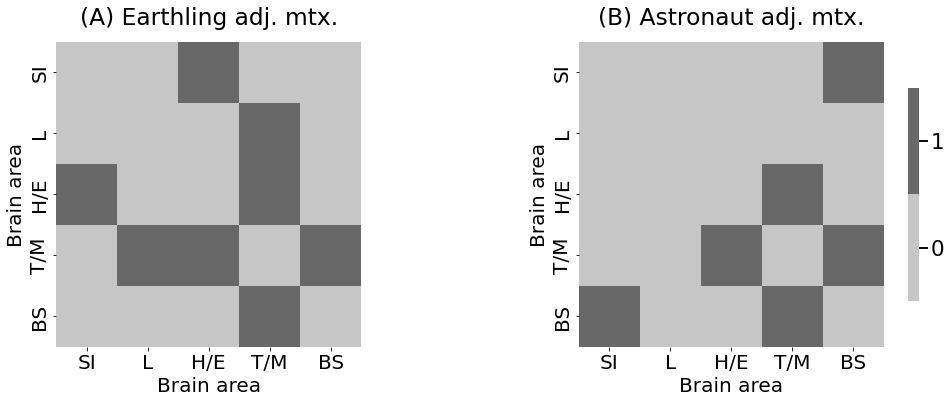
\includegraphics[width=0.7\linewidth]{representations/ch5/Images/ssg_samps.png}
    \caption[Two samples of adjacency matrices from the signal sub network model]{\textbf{(A)} a brain network of an earthling. \textbf{(B)} a brain network of an astronaut.}
    \label{fig:ch5:ssg_samps}
\end{figure}

Remember that to devise a statistical model, we view each piece of data in our sample as an observation of a corresponding random variable. When we were dealing with multiple network models, this meant that for each network $A^{(m)}$ there was a random network $\mathbf A^{(m)}$, and that this random network was the data-generating process from which we were observing $A^{(m)}$. Here, for each data pair $(A^{(m)}, y_m)$, there exists a corresponding random network $\mathbf A^{(m)}$ and a corresponding random class $\mathbf y_m$, where $(A^{(m)}, y_m)$ is a sample of $(\mathbf A^{(m)}, \mathbf y_m)$. So, for your multiple network model with covariates, we seek a model which describes both $\mathbf A^{(m)}$ and $\mathbf y_m$.

\subsection{Signal Subnetwork Model}

These astronauts are remarkably similar to the earthlings, except for one piece of information: the connections related to vision are much stronger. In other words, the \textit{subnetwork} comprised of edges incident the occipital lobe carry the \textit{signal disparity} between human and astronaut brains. This concept of a subnetwork was first explored in Section \ref{sec:ch4:prop-net:subnetwork}. 

What this means is that, if we were to just compare the adjacency matrices themselves, we would end up looking at a lot of \textit{noise}, or edges which do not show any difference between the humans and the astronauts. In a fixed sample of earthlings and astronauts, we might find disparities between these noise edges, but these disparities are just because of the particular sample of humans and astronauts that we chose and are not representative of actual differences. Rather, what we want to do is identify the subset of edges and corresponding nodes, called the \textit{signal subnetwork}, which actually carry the \textit{signal}, the set of edges which show real differences between the earthlings and the astronauts. Below, we plot the probability matrices for earthlings and astronauts:

\begin{lstlisting}[style=python]
# plot probability matrices and their differences on the same scale
heatmap(P_earthling, vmin=0, vmax=1)
heatmap(P_astronaut, vmin=0, vmax=1)
heatmap(np.abs(P_astronaut - P_earthling), vmin=0, vmax=1)
\end{lstlisting}

Which we examine in detail in Figure \ref{fig:ch5:ssg_pmtxs}. Notice that the \textit{entirety} of the disparity between earthlings and astronauts (in terms of their probability matrices) shown in Figure \ref{fig:ch5:ssg_ssn}(C) is captured by the edges which include a node involved in eyesight. We can observe this because the first row and column of the matrix (corresponding to the node for eyesight) is different between the two networks for all other pairs of nodes.

\begin{figure}
    \centering
    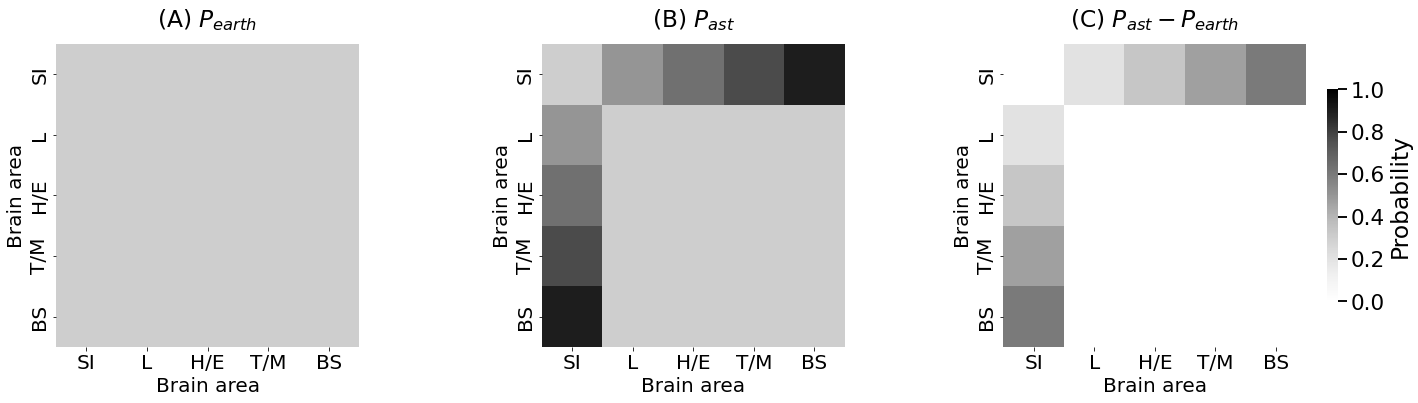
\includegraphics[width=\linewidth]{representations/ch5/Images/ssg_pmtxs.png}
    \caption[Probability matrices from two different classes]{\textbf{(A)} the probability matrix for brain networks of earthlings. \textbf{(B)} the probability matrix for brain networks of astronauts. \textbf{(C)} the difference between the probability matrices for astronauts and humans. Notice that the the area responsible for sight, SI, has very different connection probabilities with all other brain areas.}
    \label{fig:ch5:ssg_pmtxs}
\end{figure}

\subsubsection*{Signal Subnetwork}

We will attempt to explore this signal using the \textit{signal subnetwork (SSN) model}, which is a statistical model for adjacency matrices where we have a covariate. When we want to later decide whether a network is that of an earthling or an astronaut, we want to look {only} at the signal subnetwork, and ignore the rest of the network entirely.

For the SSN model, the core idea is that for each edge in the network, the probability of an edge existing (or not existing) is either the same or different between the two classes. We capture this idea using the \textit{signal subnetwork}. For an edge $(i, j)$ for classes $y$ (either $0$ or $1$), we will use the notation $p_{ij}^{(y)}$ to denote the probability of an edge existing in class $y$. 

The \textit{signal subnetwork} \cite{Vogelstein2013Jul} is a collection of edges $\mathcal S$, which has edges $(i,j)$ where $i$ and $j$ are nodes in the network between $1$ and $n$, such that the following two conditions hold:

\begin{enumerate}
    \item For each edge which is in the signal subnetwork, the probability of an edge existing differs between classes $0$ and $1$. That is, if an edge $(i, j)$ is in the signal subnetwork $\mathcal S$, then there exist two classes $y$ and $y'$ where $p_{ij}^{(y)} \neq p_{ij}^{(y')}$.
    \item For each edge which is \textit{not} in the signal subnetwork, the probabilitty of an edge existing is the \textit{same} between classes $0$ and $1$. That is, if an edge $(i, j)$ is not in the signal subnetwork $\mathcal S$, then $p_{ij}^{(0)} = p_{ij}^{(1)}$. For this reason, if an edge is not in the signal subnetwork, we will use the notation $p_{ij} = p_{ij}^{(0)} = p_{ij}^{(1)} = ... = p_{ij}^{(Y-1)}$.
\end{enumerate}

The idea is just that the signal subnetwork is keeping track of the edges which have different probabilities for any pair of classes. For our earthlings versus astronauts example above, this amounts to the set of edges for which at least one node is in the visual region of the brain:

\begin{lstlisting}[style=python]
# plot the signal subnetwork
ax = heatmap(signal_subnetwork)
\end{lstlisting}

\begin{figure}
    \centering
    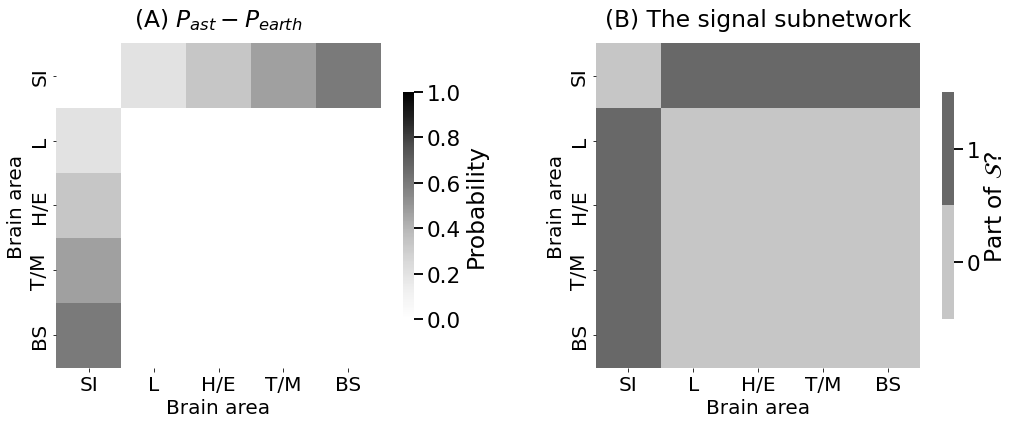
\includegraphics[width=\linewidth]{representations/ch5/Images/ssg_ssn.png}
    \caption[Signal subnetwork for earthling and astronaut examples]{\textbf{(A)} the difference between the earthling and astronaut probability matrices. \textbf{(B)} the signal subnetwork.}
    \label{fig:ch5:ssg_ssn}
\end{figure}

A plot of the signal subnetwork is shown in Figure \ref{fig:ch5:ssg_ssn}(B), and is compared to the difference between the probability matrices for earthlings and astronauts in Figure \ref{fig:ch5:ssg_ssn}(A). Notice that the signal subnetwork includes all edges in which the two probability matrices are different. 

Now that we are familiar with the signal subnetwork $\mathcal S$, we can formally define the signal subnetwork model. For each random pair $(\mathbf A^{(m)}, \mathbf y_m)$ of your $M$ total pairs, we first obtain a ``class assignment'' die with $Y$ total sides. For a given face of the dice $y$, the probability that the dice lands on side $Y$ is $\pi_y$. We flip the class assignment die, and if it lands on side $y$, then $\mathbf y_m$ takes the value $y$. Next, for each edge $(i,j)$ which is not in the signal subnetwork $\mathcal S$, we obtain a ``non-signal’’ coin which has a probability of $p_{ij}$ of landing on heads and $1 - p_{ij}$ of landing on tails. The edge $\mathbf a_{ij}$ exists if the coin lands on heads and does not exist if the coin lands on tails. Finally, for each edge $(i, j)$ which is in the signal subnetwork $\mathcal S$, we check which class $\mathbf y_m$ indicates. If $\mathbf y_m$ is class $y$, we obtain a ``signal’’ coin which has a probability of $p_{ij}^y$ of landing on heads, and a probability of $1 - p_{ij}^y$ of landing on tails. The edge $\mathbf a_{ij}$ exists if the coin lands on heads and does not exist if the coin lands on tails. 

In summary, we will say that a collection of random network/covariate pairs $\left\{(\mathbf A^{(1)}, \mathbf y_1), ..., (\mathbf A^{(M)}, \mathbf y_M)\right\}$ with $n$ nodes is $SSN_n(\pi_0, ..., \pi_{Y-1}, P^{(0)}, ..., P^{(Y-1)}, \mathcal S)$ if the following three conditions hold:
\begin{enumerate}
    \item For every edge $(i, j)$ which is in the signal subnetwork $\mathcal S$, then there exist at least two classes $y$ and $y'$ where $p_{ij}^{(y)} \neq p_{ij}^{(y')}$.
    \item For every edge $(i, j)$ which is not in the signal subnetwork $\mathcal S$, then every edge probability $p_{ij}=p_{ij}^{(1)} =...= p_{ij}^{(Y)}$. 
    \item conditional on the class $\mathbf y_m$ being $y$, then $\mathbf A^{(m)}$ is $IER_n(P^{(y)})$, where $IER_n(P^{(y)})$ is from Section \ref{sec:ch5:ier}.
\end{enumerate}

Next, let's learn how to simulate signal subnetworks.
% \subsubsection*{How do you simulate samples of $SSN_n(\pi_0, ..., \pi_{Y-1}, P^{(1)}, ..., P^{(Y-1)}, \mathcal S)$ random networks?}

\subsubsection*{How do you simulate samples of $SSN$ random networks?}

The procedure below in Algorithm \ref{alg:ch5:ssn} produce for us a set of networks, $\left\{A^{(1)}, ..., A^{(M)}\right\}$, which have nodes and edges, where the underlying random networks $\left\{\mathbf A^{(1)},..., \mathbf A^{(M)}\right\}$ are $SSN_{n,M}(\pi_0, ..., \pi_{Y-1}, P^{(1)}, ..., P^{(Y-1)}, \mathcal S)$ random networks.


\begin{algorithm}[h]\caption{Simulating samples from an $SSN_{n, M}(\pi_1, ..., \pi_Y, P^{(0)}, ..., P^{(Y-1)}, \mathcal S)$ random network}
\label{alg:ch5:ssn}
\SetAlgoLined
\KwData{$n$ a number of nodes\newline $M$ the total number of networks \newline $\pi_0,..., \pi_{Y-1}$ the probability of a network being from a given class \newline $P^{(0)}, ..., P^{(Y-1)}$ the probability matrix associated with each class \newline $\mathcal S$ the signal subnetwork}
\KwResult{A collection of $M$ networks with $n$ nodes.}

Obtain a dice with $Y$ sides numbered from $0$ to $Y-1$, that has a $\pi_y$ chance of landing on the $y$ side.

\For{$m$ in $1$:$M$} {
    Flip the $Y$-sided die, and if it lands on side $y$, assign the item $m$ to class $y$. Call this class $y^{(m)}$.

    Simulate an adjacency matrix $A^{(m)}$, using the procedure for an $IER_n(P^{(y)})$ network, in Algorithm \ref{alg:ch5:ier}.
}

\Return{$\left\{(A^{(1)}, y^{(1)}),...,(A^{(M)}, y^{(M)})\right\}$}
\end{algorithm}
